\section{Results}
RQ1: On Defects4J Java projects, does GPT-4o-mini-based mutant selection achieve a higher mutation score compared to random fixed-seed selection when both select the top 10\% of mutants?
\subsection{Overall mutation score}
\begin{table}[ht]
\centering
\caption{Overall mutation score (mutant-weighted; same budget of 1,119 mutants per branch).}
\label{tab:overall-mutation-score}
\begin{tabular}{lccc}
\hline
\textbf{Strategy} & \textbf{Selected} & \textbf{Killed} & \textbf{Mutation Score} \\
\hline
GPT-4o mini & 1,119 & 801 & \textbf{0.7158} \\
Random fixed-seed (42) & 1,119 & 750 & 0.6702 \\
\hline
\end{tabular}
\end{table}
The absolute difference is +0.0456 (+51 additional mutants killed). Project-based selection distribution (GPT): Codec 237, CSV 64, JacksonCore 818 mutants; the random selection has an identical number by group (a characteristic of by-group budgeting).
\subsection{Paired group-level (pre-registered unit)}
\begin{table*}[ht]
\centering
\caption{Paired by (project, version, class); $N = 37$ groups; one-sided Wilcoxon test; $\alpha = 0.05$.}
\label{tab:paired-results}
\begin{tabular}{lccccccccc}
\toprule
\textbf{Subset} &
\textbf{n} &
\textbf{nonzero} &
\textbf{mean MS GPT} &
\textbf{mean MS Rnd} &
\textbf{median GPT} &
\textbf{median Rnd} &
\textbf{W/L/T} &
\textbf{p} &
\textbf{$r_{rb}$} \\
\midrule
Pooled       & 37 & 26 & 0.784 & 0.725 & 0.808 & 0.714 & 17/9/11 & 0.0591 & +0.350 \\
Codec        & 13 &  8 & 0.875 & 0.829 & 0.923 & 0.923 & 4/4/5   & 0.4922 & +0.028 \\
Csv          & 10 &  6 & 0.760 & 0.682 & 0.809 & 0.733 & 4/2/4   & 0.1250 & +0.571 \\
JacksonCore  & 14 & 12 & 0.717 & 0.659 & 0.698 & 0.638 & 9/3/2   & 0.1018 & +0.436 \\
\bottomrule
\end{tabular}
\end{table*}
According to the original pre-registered criteria ($(p < 0.05 \land r_{rb} \ge 0.30 \land \text{median}(\Delta\text{MS}) > 0)$): $p=0.0591 > \alpha$ and $median(\Delta MS)=0.000 \rightarrow$ fail to reject H0; specifically, r\_rb=+0.350 (medium) reached the threshold. After the amendment (removing the median criterion), the conclusion remains unchanged because p is still $> \alpha$. No subgroup reached $p<0.05$; CSV has the largest effect size (+0.571), but n=10 (Table II).
\subsection{Tie structure and resolution}
11 out of 37 pairs were absolute ties ($\Delta MS = 0$), of which 6 pairs came from groups with $k \leq 3$ mutants selected (k distribution: min=1, median=15, max=173; 2 groups had k=1). The median of the 26 non-zero pairs was +0.082. Of the 11 ties, 8 were at MS=1.0 (both branches killed cleanly - a ceiling effect), and 1 was at MS=0.
\subsection{Robustness}
\begin{enumerate}[label=(\alph*)]
    \item Mutant-weighted two-proportion z-test: difference +0.0456; z=2.34; p=0.0097 $\rightarrow$ reject H0 at the mutant level.
    \item Monte Carlo simulation (5,000 random by-group selections under the same budget): the overall MS distribution for random selection has mean=0.6700, sd=0.0126, and range [2.5\%; 97.5\%] = [0.6452; 0.6935]. GPT's MS (0.7158) is +3.64 sd above the mean; only 1/5,000 draws achieved $\geq$ GPT's score $\rightarrow$ experimental p=0.0002. Seed 42 (the pre-registered baseline) falls at the 52nd percentile of the distribution - a typical draw.
    \item NO\_COVERAGE control: the NO\_COVERAGE rate in the GPT sample was 20.7\% compared to 21.8-23.5\% for random selection; on the covered-only subset, MS was 0.864 (GPT) vs. 0.810 (random seed 42) - the advantage did not come from avoiding uncovered mutants.
    \item Source of the difference: the +51 additional mutant kills show strong concentration - the 3 largest JacksonCore groups (UTF8StreamJsonParser 3f/9f, ReaderBasedJsonParser 9f) contributed 32/51 = 63\%; the single group with the largest difference was Codec 6f Base64InputStream (+0.75, k=4). The average percentage of groups in which GPT completely won across the Monte Carlo simulations was only 46.1\%.
\end{enumerate}

\begin{figure}[ht]
\centering
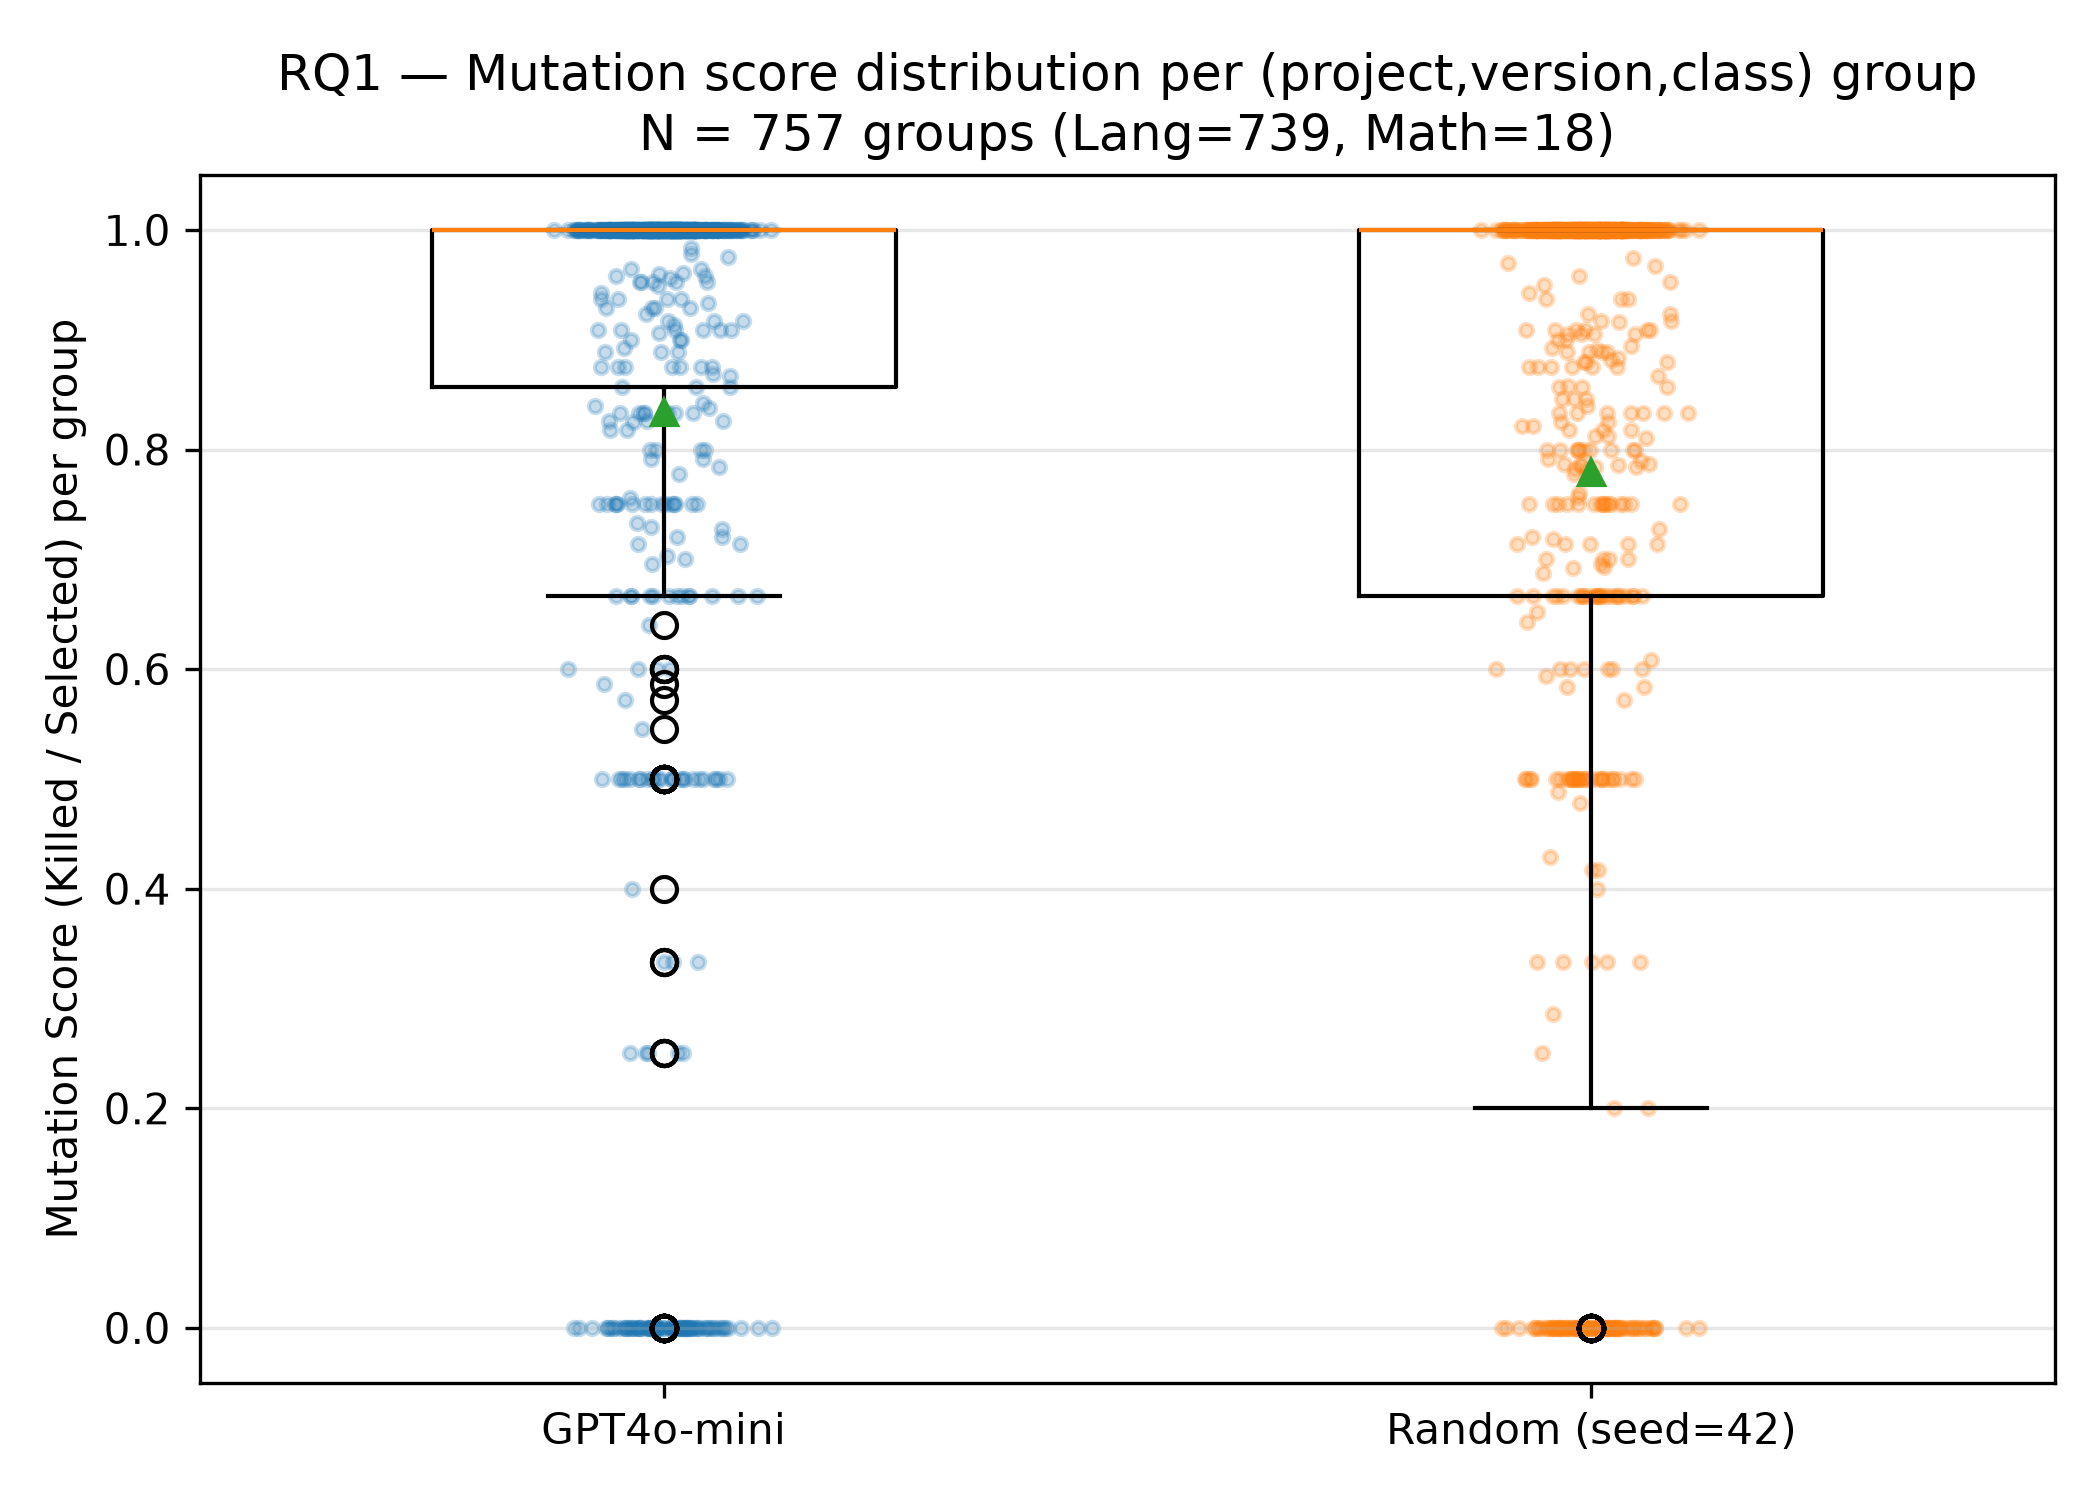
\includegraphics[width=\linewidth]{figures/fig1_distribution.png}
\caption{Boxplot showing the MS distribution per group by strategy.}
\label{fig:distribution}
\end{figure}

\begin{figure}[ht]
\centering

\includegraphics[width=\linewidth]{figures/fig2_comparison.png}
\caption{Mean MS by project, with N annotation.}
\label{fig:comparison-by-project}
\end{figure}